%%%%%%%%%%%%%%%%%%%% Documentación del usuario %%%%%%%%%%%%%%%%%%%%


\section{Documentación de usuario}

Documentación relacionada con las funciones del sistema 
pero no se hace referencia a nada relativo a su implementación. 
Está orientado a las personas que van a usar el sistema no a los 
que lo van a mantener.

\subsection{Descripción funcional}

En esta sección se procederá a describir las funcionalidades disponibles, aportar 
información sobre las posibles formas de desarrollo de una partida e informar sobre 
todo lo que se puede esperar del programa.

\bigskip

Nuestra implementación de \textbf{ESI-Escape} tiene como propósito proporcionar 
una experiencia de juego que incluya las siguientes características:

\begin{itemize}
  \item \textbf{Interacción con el usuario}: Se proporciona una interfaz gráfica de juego, que consiste en textos y mensajes desencadenados por el flujo
  del juego, que informan en todo momento al usuario del estado de las decisiones que toma, como por ejemplo desplazarse o coger un objeto,
  así como de las funcionalidades que tiene disponibles durante la partida.
  \item \textbf{Interacción con objetos}: Esto es poder recoger objetos y añadirlos a un \emph{inventario} perteneciente a un jugador, una representación 
  abstracta de los objetos que puede usar para resolver puzles y poder situarlos en salas concretas durante la partida.
  \item \textbf{Resolución de Puzles}: Es posible insertar un puzle en una sala en base a un archivo de configuración y asociarlo al desbloqueo 
  de una conexión entre dos salas concretas. Este puzle podría consistir en la introducción de un código o una palabra que podrías encontrar a través de
  pistas que el propio juego proporciona. Esto vendría configurado
  \item \textbf{Generación personalizada de un mapa}: Se permite la creación de un número extensible de salas y conexiones a través de una 
  cadena en un formato concreto ubicada en los ficheros de configuración asociados a este propósito y descritos en detalle más adelante en la documentación.
  \item \textbf{Registro de jugadores}: Es posible albergar múltiples jugadores almacenadas mediante una tupla \emph{Usuario-Contraseña} que se
  creará a través de una función de registro, que será lo primero que un usuario encuentre al iniciar el programa.
  \item \textbf{Persistencia de los datos}: Es posible guardar tu partida durante el juego, quedando almacenada en un fichero de configuración 
  del cual más tarde puede recuperarse en base a tu usuario y contraseña. Nuestra implementación solo permite una partida guardada
  por jugador, que se irá sobreescribiendo con cada guardado.
\end{itemize}

En la siguiente figura podemos observar un esquema que nos informa del 
flujo general del programa:

{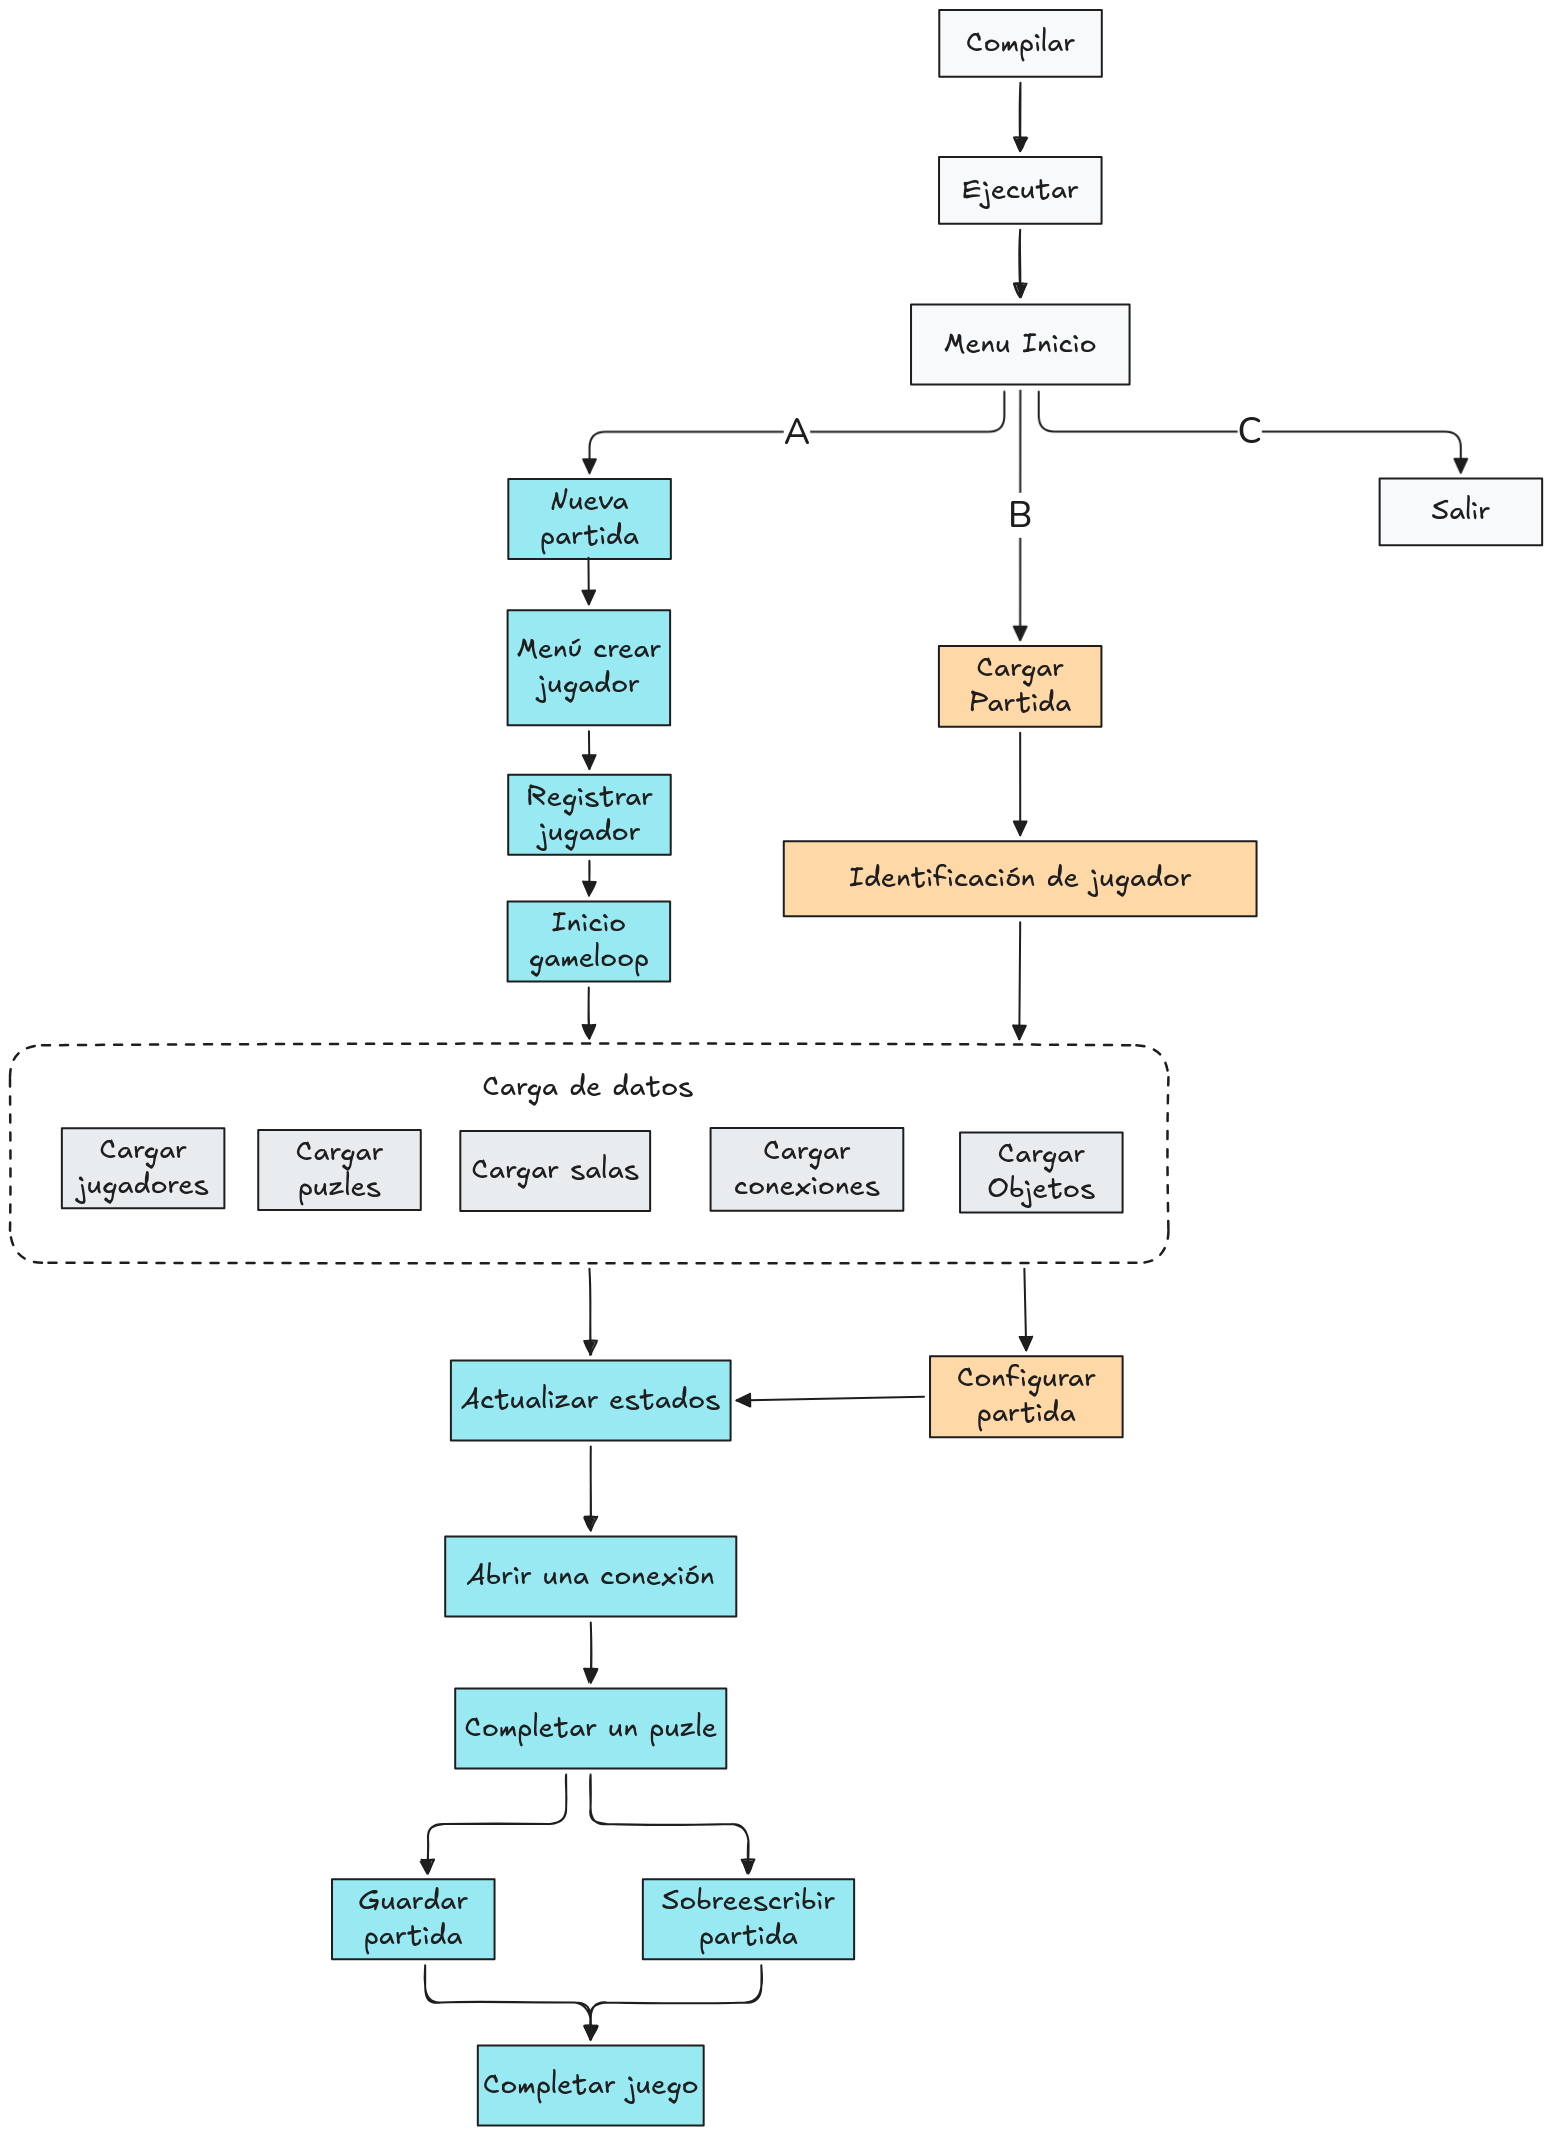
\includegraphics[width=1\textwidth]{gameFlow.png}}\\[1\baselineskip]

\newpage

Pueden distinguirse \textbf{tres ramas principales}, que hemos llamado \emph{A,B y C},
basadas en las posibles elecciones desde el menú principal.

\bigskip

La rama \emph{A}, la más más natural, consiste en iniciar una partida nueva, 
registrar tu jugador,y a partir de ese momento el bucle principal del juego se inicia, 
permitiéndonos ya interactuar con las salas, los objetos y los puzles.

\bigskip

La rama \emph{B} consiste en seleccionar la opción "\textbf{Cargar partida}", 
que considera la existencia de un perfil de jugador, pide identificación mediante 
usuario y contraseña para luego entrar en el flujo \emph{A}, con la diferencia de que
antes de hacerlo se añade el paso extra de "\textbf{Configurar partida}", donde se 
establece en memoria el estado guardado de la partida anterior.

\bigskip

La tercera rama \emph{C}, es simplemente salir del programa.

\bigskip

En nuestra entrega del proyecto se incluye una configuración de salas y objetos 
simplificada para facilitar la revisión de la misma, consiste
en el siguiente mapa de juego:

\bigskip

{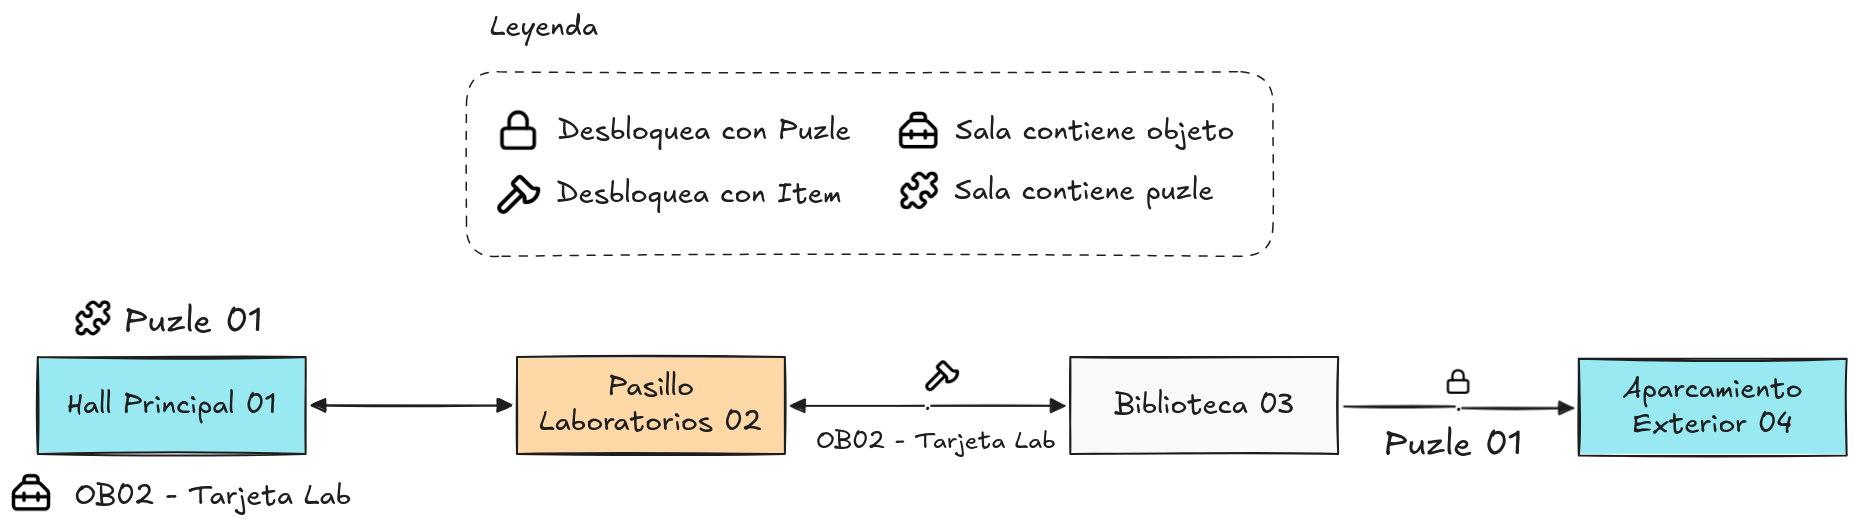
\includegraphics[width=1\textwidth]{Map.png}}\\[1\baselineskip]

Hemos optado por este diseño para poder incluir todas las funcionalidades 
en la menor cantidad de salas posibles.

\subsection{Tecnologías}

Las tecnologías y herramientas usadas para el desarrollo de este proyecto de juego de escape-room son:
\begin{itemize}

	\item \textbf{Git}: Usado para la administración de los archivos del proyecto, control de versión, y compartido de archivos para trabajo en equipo.
	\item \textbf{GitHub}: Plataforma de desarrollo donde se ha alojado el repositorio de \emph{Git} y se ha realizado la planificación del proyecto mediante su herramienta \emph{GitHub Projects}.
	\item \textbf{Visual Studio Code}: Editor de código con integración de Git para ver los cambios realizados y resolver conflictos donde varios miembros del equipo suban modificaciones que colisionen una con la otra.
	\item Librerías: 
	\begin{itemize}
		\item Se usan las librerías \textbf{del estándar ANSI C}, las cuales son empleadas para constituir módulos que realizan las distintas tareas que requiere el proyecto.
		\item \textbf{Doxygen} para la generación de documentación automática a partir de los comentarios del código fuente.
	\end{itemize}
\end{itemize}


\subsection{Manual de instalación}

Para la instalación de nuestra implementación de ESI-Escape, el usuario deberá ejecutar desde la terminal \textbf{(¡MUY IMPORTANTE, hacerlo estando dentro del directorio del proyecto, para asegurar la carga de archivos con las rutas correctas!)} ''run'' (para directamente ejecutar el proyecto si está ya compilado en la carpeta "bin"), ''run\_and\_compile'' (para compilar el proyecto y luego ejecutarlo) o ''compile'' (para solo compilarlo en la carpeta ''bin''). Se usarán los archivos .bat si el usuario se encuentra en el sistema operativo Windows y los archivos .sh si se encuentra en Linux.

\bigskip

Para la compilación, es necesario que el usuario tenga instalado ''make'' mediante la forma preferida y disponible del usuario (en Linux lo instalamos usando el administrador de paquetes preferido para instalar ''build\_essential'', pero cabe notar que la instalación de esta herramienta varía dependiendo del tipo de distribución, y muchas veces viene preinstalada), y en Windows que tenga instalado ''MinGW'' con su carpeta ''bin'' añadida al PATH para la llamada que hacen ''run\_and\_compile'' y ''compile'' de ''mingw32-make'', el cual cumple la misma función que ''make'': compilar todo el proyecto con sus archivos de cabecera .h y de código .c.

\bigskip

\textbf{(Los archivos .txt de datos de entrada y de guardado de partida y jugadores se encuentran en el directorio ''data'').}

\subsection{Acceso al sistema}

Al entrar al programa, se le pedirá al usuario introducir su nombre de acceso y contraseña. Si estos no son encontrados, se le ofrece el usuario registrarse, pidiendo adicionalmente un nombre completo para este. Una vez iniciado sesión, el usuario verá el menú de inicio de ESI-ESCAPE, con las opciones de comenzar una Nueva partida, Cargar partida y Salir (para salir del juego de vuelta al sistema operativo). Durante una partida, la opción "Volver" te permitirá salir al menú de inicio para entonces dejar el juego.

\bigskip

El usuario se puede encontrar con el problema de encontrarse mensajes de alerta con archivos los cuales no pudieron ser cargados. En esos casos, la solución radica en ejecutar ''run'' o ''run\_and\_compile'' situándonos con la terminal en la carpeta del proyecto (es decir, la misma que contiene dichos archivos), para que así ESI-Escape encuentre los archivos .txt.

\bigskip

También puede ocurrir que el sistema operativo no encuentre ''bin/esi-escape'' o ''mingw32-make'' o "make".
\begin{enumerate}
	\item Si no se encuentra ''bin/esi-escape'' al ejecutar ''run'', significa que no está compilado, o no se está ejecutando ''run'' o ''run\_and\_compile' desde la carpeta del juego'. Se soluciona ejecutando ''run'', ''run\_and\_compile'' o ''compile'' desde la carpeta del juego, y asegurándonos de que el ejecutable está presente en ''bin'' haciendo ''run\_and\_compile'' o ''compile''.
	\item Si no se encuentra ''mingw32-make'', instalar MinGW en tu equipo Windows, o si estás usando Linux, es recomendable instalar ''make'' en su lugar mediante la forma preferida y disponible del usuario (en Linux lo instalamos usando el administrador de paquetes preferido para instalar ''build\_esential'').
	\item Si no se encuentra ''make'', y estando en Linux, lo instalamos mediante la forma preferida y disponible del usuario (en Linux lo instalamos usando el administrador de paquetes preferido para instalar ''build\_essential'', pero cabe notar que la instalación de esta herramienta varía dependiendo del tipo de distribución, y muchas veces viene preinstalada).
\end{enumerate}

\subsection{Manual de referencia}

La interfaz de juego de ESI-Escape permite una navegación fluida entre las salas y sus objetos y puzles; permitiendo realizar diversas acciones sobre estos.
\bigskip
\begin{itemize}
	\item Las opciones de ''Describir sala'', ''Examinar (objetos y salidas)'' e ''Inventario'' mostrarán información sobre lo que sus nombres indican, para luego pedir al usuario una pulsación para volver al menú de juego.
	\item ''Entrar en otra sala'' te permitirá ir a otra sala la cual no esté bloqueada, esté adyacente a la actual y exista.\bigskip

''Coger objeto'' te permitirá agarrar un objeto que exista y esté presente en la sala actual.\bigskip

''Soltar objeto'' permite colocar un objeto que exista y esté en tu inventario en la sala actual.\bigskip

''Usar objeto'' permite usar un objeto que exista y esté en tu inventario para desbloquear salidas que requieran de dicho objeto para desbloquearse, estén adyacentes a la actual y existan.\bigskip

Y ''Resolver puzle / introducir código'' permite al usuario resolver un puzle o introducir un código que exista y se encuentre en la sala actual, para así desbloquear las salidas que lo tengan como condición en cualquier parte.\bigskip

\textbf{Si cualquiera de las condiciones especificadas anteriormente no se cumplen, el juego mostrará mensajes de error haciendo saber al jugador lo que está incumpliendo.}

\item Al pulsar ''Guardar partida'', los datos de la partida actual son almacenados en el directorio ''data'' para que el usuario pueda cargar su partida en una próxima sesión.

\item Por último, si pulsas ''Volver'', el usuario volverá a la pantalla de inicio donde podrá crear una Nueva partida, Cargar partida o Salir del juego.

\end{itemize}

\subsection{Guía del operador}

(Este programa no requiere de operador)